\documentclass[oneside]{book}
\usepackage[utf8]{inputenc}
\usepackage{fancyhdr}
\usepackage[spanish]{babel}
\usepackage[document]{ragged2e}
\usepackage{lastpage}
\usepackage{amsmath}
\usepackage{listings}
\usepackage{xcolor}
\usepackage{enumitem}
\usepackage{siunitx}
\usepackage{amssymb}
\usepackage{mathrsfs, amsmath}
\usepackage{amsfonts}
\usepackage{amsthm}
\usepackage{tcolorbox}
\usepackage{cancel}
\usepackage{siunitx}
\usepackage{nccmath}
\usepackage{hyperref,lipsum}
\usepackage{ragged2e}
\usepackage{fullpage}

\lstset{
    language=R,
    basicstyle=\ttfamily\small,
    keywordstyle=\color{blue},
    stringstyle=\color{red},
    commentstyle=\color{gray},
    showstringspaces=false,
    breaklines=true,
    backgroundcolor=\color{lightgray}, % <<< fundo cinza
    frame=single,                      % <<< borda ao redor
    literate={_}{{\_}}1                % <<< tratar "_" normalmente
}




\setlength{\headheight}{12.0pt} % Set the headheight to at least 12.0pt
\addtolength{\topmargin}{-12.0pt} % Adjust topmargin to compensate

\pagestyle{fancy}
\fancyhf{}
\newcommand{\Lagr}{\mathcal{L}}
\lhead[Head 1]{P1 de Astroestatística}
\rhead[Head 2]{Iago Lopes}
\rfoot[Página \thepage]{Página \thepage}
\begin{document}

\begin{titlepage}
\centering
{\bfseries\LARGE Universidade Federal do Rio de Janeiro \par}
\vspace{0.1cm}
{\bfseries\LARGE Observatório do Valongo \par}
\vfill
\noindent\hrulefill \\
{\scshape\Huge Primeira prova\par} %Título
\vspace{0.5cm}
{\scshape\Large Astroestatística \par}
\vspace{0.5cm}
{\scshape\Large 2025.1 \par} %Semestre
\noindent\hrulefill \\
\vfill
{\bfseries\Large Iago Lopes\\ \small DRE: 122077032 \par}
\vfill
{\Large Professor: Hélio Jaques \par}
\vfill
{\large 31 de Maio de 2025 \par} %esto crea la fecha de hoy
\end{titlepage}
\setcounter{page}{1}
\newpage
{$\space$\par}
\vspace{0.5cm}
\justifying
\section*{{\bfseries \LARGE Questão 1 -} {\bfseries \large  Represente cada aluno por uma Face de Chernoff. A partir delas, você julga que há alunos que apresentem um histórico no ENEM e CRA do primeiro período similar entre si? Ou não?}}

\vspace{0.2cm}

\textcolor{red}{Um bom método para exploração e classificação é o de Faces de Chernoff que utiliza característica físicas para exemplificar o quão similar os dados são no espaço de seus parâmetros. Duas faces similares indicam pontos que estão em uma região próxima no espaço dos parâmetros. Esse método facilita para humanos avaliarem similaridades nos dados e então poder trabalhar em cima dessa análise inicial. Para isso usei a função \texttt{faces} considerando todas as colunas da amostra de alunos da astronomia, exceto seus nomes e o ano da turma, já que não são relevantes ao olhar para a nota do Enem e o CRA.}

\vspace{0.2cm}

\begin{lstlisting}
    install.packages('TeachingDemos')
    library(TeachingDemos)

    astro = read.table('/content/ENEM_Astro.csv', sep=',', header=T)
    
    options(repr.plot.width=14,repr.plot.height=12)
    # Usando todas colunas, exceto o nome para criar as faces
    faces(astro[, 2:7], labels = astro$Nome)
\end{lstlisting}


\begin{figure}[h]
    \centering
    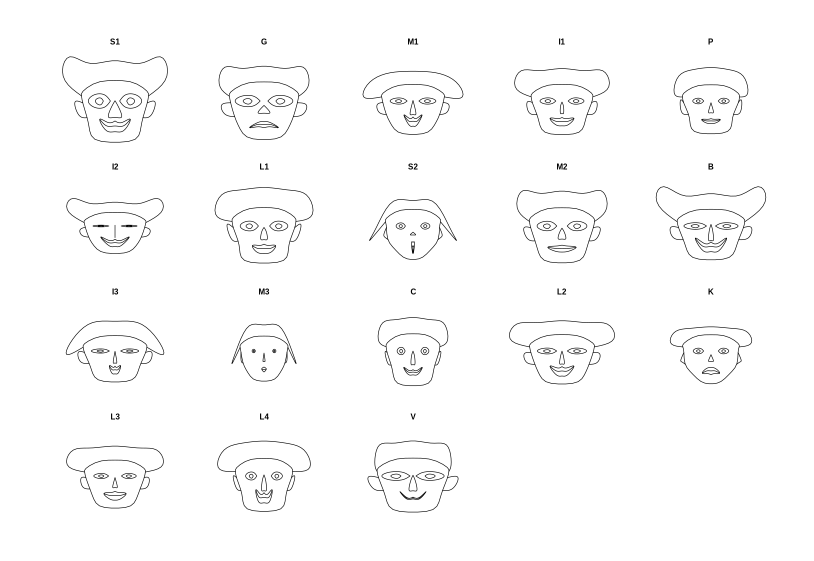
\includegraphics[width=0.8\linewidth]{Figuras/Faces.png}
    \caption{Resultado ao aplicar o método de faces de Chernoff na amostra de alunos da astronomia.}
    \label{faces}
\end{figure}

\textcolor{red}{O resultado pode ser visto na imagem \ref{faces}, onde é possível dizer que de fato há alunos similares nesse espaço de parâmetros. Os principais grupo que percebi foi o de: (S1, B), (S2, M3) e (L1, L2, L3) como indicado na imagem.}
\newpage
{$\space$\par}
\vspace{0.5cm}
\justifying
\section*{{\bfseries \LARGE Questão 2 -} {\bfseries \large A figura abaixo representa medições de rádio feitas pelo radiotelescópio Big Ear em 1977. As observações destacadas pelo círculo vermelho onde se lê 6EQUJ5 ficaram conhecidas como Sinal Uau (ou Wow, como quiser). As letras e números representam uma escala de intensidade, segundo a ordem: 123456789ABCDEFGHIJKLMNOPQRSTU. A cada 2 segundos, a intensidade do sinal medido seria representada por uma dessas letras. Suponha que essa escala seja linear, tal que 1 represente intensidade 1, 7 represente intensidade 7, A represente intensidade 10, e assim por diante, até a letra U, que representa a intensidade 30. Cada coluna composta por um caracter representa uma série de medidas. Com base nos dados dessa figura, estime a probabilidade
do Sinal Uau ter sido um evento
aleatório.}}

\vspace{0.2cm}

\begin{figure}[h]
    \centering
    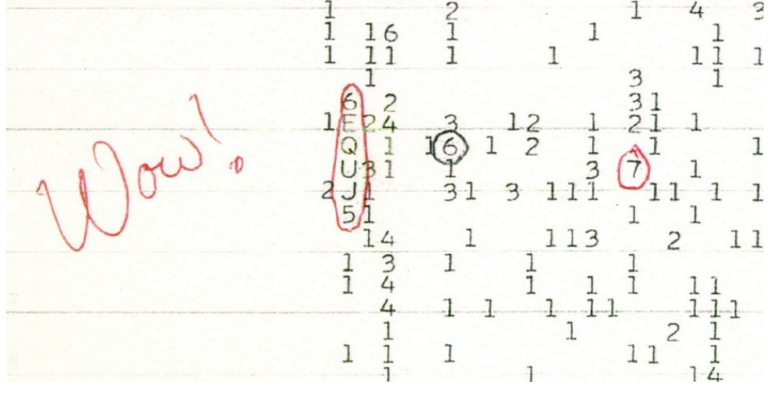
\includegraphics[width=0.5\linewidth]{Figuras/Captura de tela 2025-06-01 094035.png}
\end{figure}

\vspace{0.8cm}

\textcolor{red}{Este é um problema comum na astronomia e para resolvê-lo usarei a distribuição de Poisson, pois a intensidade é uma contagem de fótons, fazendo que essa distribuição seja a mais adequada para o problema. Para verificar se o evento Uau é um sinal aleatório, primeiro vou estimar a média das outras observações, ou seja, o $\lambda$ da distribuição de Poisson.} 

\textcolor{red}{Aqui vou assumir que os espaços vazios são intervalos de 2 segundos onde não houve nenhum fóton, logo sua intensidade será 0, e também vou desconsiderar a coluna do evento Uau nessa estimativa. Considerando 22 colunas e 17 linhas, temos:}

\vspace{0.8cm}

\begin{lstlisting}
    values_no_wow_no_zero = c(rep(1,77), rep(2,8), rep(3,10), rep(4,6), rep(6,2), rep(7,1))
    
    values_no_wow = c(values_no_wow_no_zero, rep(0,17*22-length(values_no_wow_no_zero)))

    lambda = mean(values_no_wow)
\end{lstlisting}

\textcolor{red}{Isso resulta em $\lambda\approx0.444$, ou seja, em média temos $0.444$ de intensidade a cada $2$ segundos. Agora, podemos estimar a probabilidade de ocorrer 6EQUJ5 ou mais do que isso em 12 segundos:}
$$
I_{med} = \frac{6 +14+ 26+ 30+ 19+ 5}{6}\approx16.66
$$
$$
P(x>I_{med}) = \int_{I_{med}}^\infty \frac{e^{-\lambda}\lambda^x}{x!} dx
$$
\textcolor{red}{A partir disso, podemos estimar a probabilidade de que isso seja um evento aleatório, usando:}
$$
P_{aleatorio} = 1-P(x>I_{med})=1.862e-21
$$

\begin{lstlisting}
    wow = c(6, 14, 26, 30, 19, 5)
    prob = ppois(mean(wow), lambda=lambda, lower.tail = F)
\end{lstlisting}

\textcolor{red}{Logo, podemos dizer que a probabilidade de que isso seja um evento aleatório é praticamente nula e que é altamente provável que esse evento seja algum fenômeno físico a ser investigado.}
\newpage
{$\space$\par}
\vspace{0.5cm}
\justifying
\section*{{\bfseries \LARGE Questão 3 -} {\bfseries \large  Um determinado modelo de formação estelar prevê que cerca de 38\% das estrelas de um aglomerado globular devem ser binárias. Seu colaborador estudou 568 estrelas de um aglomerado globular e encontrou que 200 delas devem ser binárias. Com base nesses dados, você pode refutar o modelo mencionado acima?}}

\vspace{0.8cm}

\textcolor{red}{Para isso, precisamos utilizar um teste de hipótese baseado em proporções, que é o mais adequado ao problema:}

\vspace{0.4cm}

\begin{lstlisting}
    prop.test(200, n = 568, p=0.38)
\end{lstlisting}

\begin{lstlisting}
    	1-sample proportions test with continuity correction
    
    data:  200 out of 568, null probability 0.38
    X-squared = 1.7584, df = 1, p-value = 0.1848
    alternative hypothesis: true p is not equal to 0.38
    95 percent confidence interval:
     0.3130942 0.3931624
    sample estimates:
            p 
    0.3521127 
\end{lstlisting}

\vspace{0.4cm}

\textcolor{red}{De acordo com o teste de proporções, não podemos refutar o modelo mencionado, pois seu p-valor é de $0.38$ e nessa análise estamos considerando como evidência forte valores p menores do que $0.05$.}
\newpage
{$\space$\par}
\vspace{0.5cm}
\justifying
\section*{{\bfseries \LARGE Questão 4 -} {\bfseries \large  Compare a densidade das notas obtidas pelos alunos de 2024 com as de 2025 em uma figura com 6 paineis, um para cada nota. As distribuições são estatisticamente similares entre os alunos de cada ano?.}}

\vspace{0.2cm}

\textcolor{red}{Se buscamos verificar a similaridade estatística entre as distribuições de cada ano, precisamos de testes estatísticos que nos permitam realizar afirmações. Nessa sitaução, utilizei 4 testes: t-test, F-test, KS-test, Wilcox-test. A escolha dos testes foi feita de maneira que seja possível testes diferentes características das amostras. Além disso, decidir fazer um teste utilizando a MANOVA, ou seja, considerando a mediana de todas as dimensões ao mesmo tempo e obtive um valor p de: 0.49}

\begin{lstlisting}
    par(mfcol = c(3, 2)) 
    
    colors = c('blue', 'red')
    for (i in 2:7) {  
      values_1 = astro[astro$ano == 2025, i]
      values_2 = astro[astro$ano == 2024, i]
    
      # Tests
      t_test = t.test(values_1, values_2)
      f_test = var.test(values_1, values_2)
      ks_test = ks.test(values_1, values_2)
      wil = wilcox.test(values_1, values_2, exact = FALSE)
    
      # Plot
      plot(density(values_1), col = colors[1], xlab = 'Pontuação',
           main = colnames(astro)[i], ylim = c(0, max(density(values_1)$y,
            density(values_2)$y) * 1.2))
      lines(density(values_2), col = colors[2])
    
      # Add text
      text_x = median(median(values_1),median(values_2)) *0.8
      y_start = 0.008
    
      text(text_x, y_start*0.9,     paste("t: ", round(t_test$p.value, 3),
      "\nF: ", round(f_test$p.value, 3),
      "\nKS: ", round(ks_test$p.value, 3),
      "\nWil: ", round(wil$p.value, 3)), pos = 3)
    }
    
    legend('topleft', legend = c(2025, 2024), col = colors, lty = 1, bty = 'n', 
    cex = 1.2)
    # MANOVA
    man_test = manova(as.matrix(astro[,2:7]) ~ astro$ano)
    cat("\nMANOVA teste para todas as áreas:\n")
    print(summary(man_test))
\end{lstlisting}

\begin{figure}[h]
    \centering
    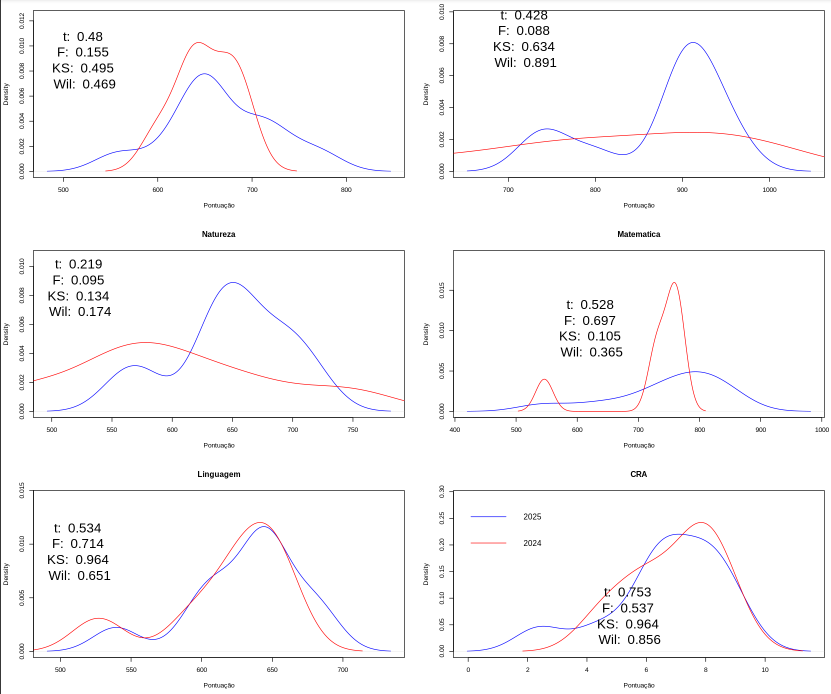
\includegraphics[width=1\linewidth]{Figuras/grades.png}
    \caption{Distribuição da notas dos alunos da astronomia classificados por ano de ingresso junto com o valor p dos 4 testes estatísticos escolhidos para a análise.}
    \label{grades}
\end{figure}

\vspace{8em}

\textcolor{red}{Ao olhar o resultado de diferentes testes na figura \ref{grades}, não podemos afirmar que as distribuições são de diferentes populações. Portanto, pode-se dizer que são estatisticamente similares.}

\newpage
{$\space$\par}
\vspace{0.5cm}
\justifying
\section*{{\bfseries \LARGE Questão 5 -} {\bfseries \large  Estime os parâmetros das leis de potência que descrevem: 
\begin{enumerate}
    \item a distribuição de massas das estrelas primárias (M1);
    \item  a distribuição de massa das estrelas secundárias (M2). Represente ambas as distribuições empíricas em um gráfico quantil-quantil.
\end{enumerate}}}

\vspace{0.8cm}

\textcolor{red}{A distribuição de Pareto é muito utilizada em astronomia devido às diferentes escalas envolvidas na área. Nessa amostra de dados, temos a massa das estrelas de vários sistemas binários em logaritmo. Para estimar os parâmetros dessas leis de potência, vou utilizar o método de mínimos quadrados:}

\vspace{0.8cm}

\begin{lstlisting}
    binaries = read.table('/content/belikov.dat', header=T, sep='|')

    pareto.MLE = function(X) {
      n = length(X)
      m = min(X)
      a = n/sum(log(X)-log(m)) 
      return(c(m,a))
      
    # Fitting
    params_m1 = pareto.MLE(10**binaries$M1)
    params_m2 = pareto.MLE(10**binaries$M2)
    cat('Fit for primary stars (location, shape):',params_m1[1],params_m1[2],'\n')
    cat('Fit for secundary stars (location, shape):',params_m2[1],params_m2[2])

    # Creating theoretical values from fitted distribution
    fit_m1 = log10(rpareto(length(binaries$M1), shape=params_m1[2], scale=params_m1[1]))
    fit_m2 = log10(rpareto(length(binaries$M2), shape=params_m2[2], scale=params_m2[1]))

    # QQ plot for Primaries
    qqplot(binaries$M1, fit_m1, xlab = "Primary mass (log)", ylab = "Primary mass from fit (log)")
    lines(binaries$M1, binaries$M1, col='red', lwd=4)
    legend('topleft', legend='Q_empirical = Q_fitted', lwd=4, col='red', box.lwd=0)

    # QQ plot for secundaries
    qqplot(binaries$M2, fit_m2, xlab = "Secundary mass (log)", ylab = "Secundary mass from fit (log)")
    lines(binaries$M2, binaries$M2, col='red', lwd=4)
    legend('topleft', legend='Q_empirical = Q_fitted', lwd=4, col='red', box.lwd=0)
}
\end{lstlisting}

\begin{lstlisting}
    Fit for primary stars (location, shape): 1.16681 0.1031938 
    Fit for secundary stars (location, shape): 1.135011 0.1446229
\end{lstlisting}

\begin{figure}
    \centering
    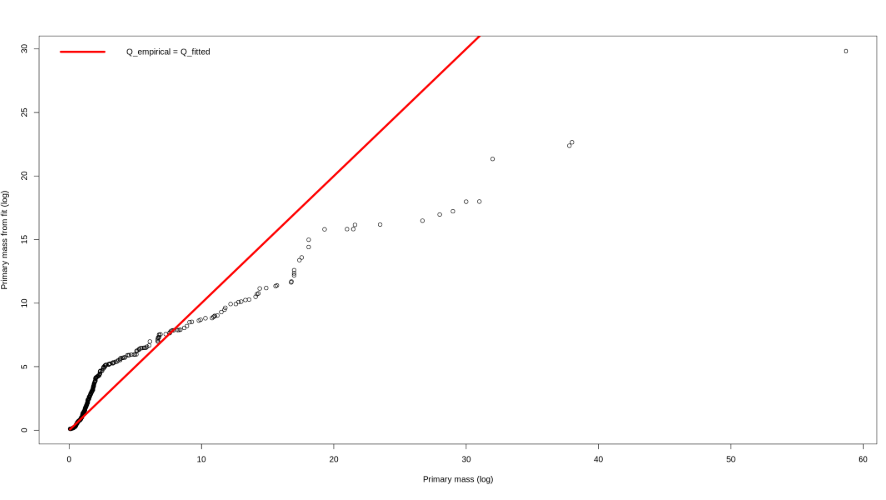
\includegraphics[width=0.9\linewidth]{Figuras/Captura de tela 2025-06-01 113313.png}
    \caption{QQ plot com a massa primaria no eixo x e Pareto ajustada no eixo y. A linha vermelha representa o caso onde os quantis dos dados e da distribuição ajustada são iguais.}
\end{figure}

\begin{figure}
    \centering
    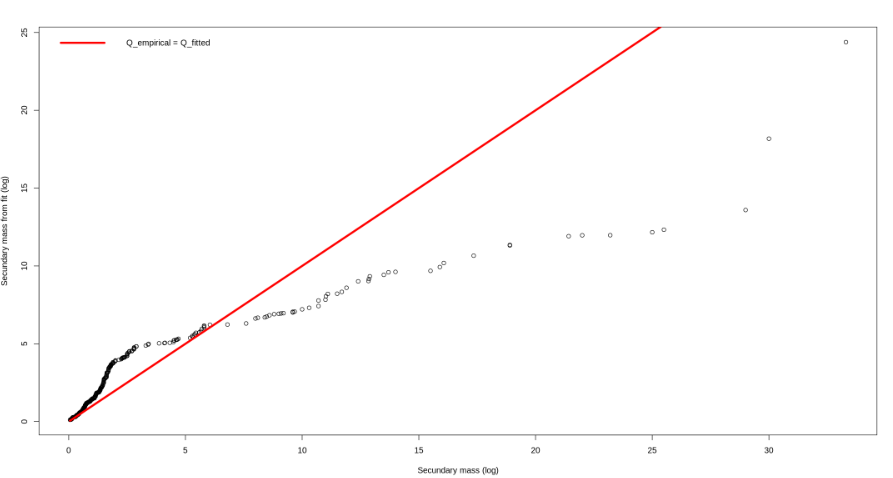
\includegraphics[width=0.9\linewidth]{Figuras/Captura de tela 2025-06-01 113326.png}
    \caption{QQ plot com a massa secundária no eixo x e Pareto ajustada no eixo y. A linha vermelha representa o caso onde os quantis dos dados e da distribuição ajustada são iguais.}
\end{figure}
\newpage
{$\space$\par}
\vspace{0.5cm}
\justifying
\section*{{\bfseries \LARGE Questão 6 -} {\bfseries \large Transforme as cores em magnitudes U, B, R e I, e junte essas magnitudes à V em uma nova dataframe. Aplique a técnica de componentes principais nesta dataframe formada apenas por magnitudes aparentes.}}

\vspace{0.3cm}

\begin{enumerate}
    \item Quantas componentes principais poderiam explicar apropriadamente a distribuição das estrelas nesse espaço de magnitudes?
        
    \item Interprete. O que deve significar fisicamente os dois primeiros componentes principais?

    \item Quais seriam as magnitudes de uma estrela hipotética que pudesse ser representada no espaço de componentes principais pelas coordenadas (0.2, 0.43, 0.6, 0.8, 0.4)?
\end{enumerate}
\vspace{0.8cm}

\textcolor{red}{O método de PCA rotaciona o espaço dos parâmetros de maneira que os primeiros eixos sejam aqueles onde há maior variância dos dados. Esse método é muito útil para reduzir a dimensionalidade do problema ao assumir que as componentes de menor variância são ruídos.}

\vspace{0.4cm}

\begin{lstlisting}
    catalog = read.table('/content/king5.tsv', sep='|', header=T)

    # Estimating magnitude
    Bmag = catalog$BV+catalog$Vmag
    Umag = catalog$UB+Bmag
    Rmag = -(catalog$VR-catalog$Vmag)
    Imag = -(catalog$VI-catalog$Vmag)
    
    new_df = data.frame(Umag = Umag, Bmag = Bmag, Vmag = catalog$Vmag, Rmag = Rmag,
     Imag = Imag
    )
    new_df = new_df[complete.cases(new_df),]
    
    # PCA
    pca = prcomp(new_df)
    summary(pca)
    
    ### output ### 
    Importance of components:
                              PC1     PC2     PC3     PC4     PC5
    Standard deviation     2.7876 0.42396 0.17145 0.04079 0.03337
    Proportion of Variance 0.9735 0.02252 0.00368 0.00021 0.00014
    Cumulative Proportion  0.9735 0.99597 0.99965 0.99986 1.00000
\end{lstlisting}

\textcolor{red}{a) Vemos que as duas primeira componentes já conseguem explicar mais de $99.5\%$ da variância, portanto eu diria que duas componentes principais já são suficientes para explicar os dados.}


\begin{lstlisting}
    par(mfrow=c(2,1))
    barplot(pca$rotation[,1]) # Brilho
    barplot(pca$rotation[,2]) # Cor
\end{lstlisting}

\textcolor{red}{b) Para interpretar, decidi fazer um gráfico de barras das componentes e percebi que a primeira componente está relacionada simplesmente com a magnitude das estrelas, ou seja, o brilho aparente delas. Já para a segunda componente, notei que as banda U e I estão com maior peso, logo imagino que essa componente está buscando explicar as cores das estrelas, ou seja, suas temperaturas efetivas, pois se a T$_{eff}$ é baixa, então emitirá mais em comprimentos de onda maiores, enquanto que para T$_{eff}$ alta, temos maior emissão em comprimentos de onda menores.}


\textcolor{red}{c) Para computar as magnitudes nesse espaço, basta utilizar os coeficientes, ou seja, aplicar a transposta da matriz no vetor do espaço do PCA.}

\begin{lstlisting}
    pca_vector = c(0.2, 0.43, 0.6, 0.8, 0.4)
    mags = c()
    for (i in c(1:5)){
      mag = sum(pca$rotation[i,] * pca_vector) + mean(new_df[,i])
      mags = c(mags,mag)
    }
    cat('Magnitudes (U,B,V,R,I): ',mags)

    ### output ###
    Magnitudes (U,B,V,R,I):  19.74012 17.93687 17.82269 16.01448 16.04089
\end{lstlisting}


\newpage
{$\space$\par}
\vspace{0.5cm}
\justifying
\section*{{\bfseries \LARGE Questão 7 -} {\bfseries \large Aplique uma decomposição de misturas às magnitudes U, B, V, R e I do aglomerado King 5 considerando que cada componente seja uma normal multivariacional.
}}

\vspace{0.3cm}

\begin{enumerate}
    \item Quantas componentes normais multivariacionais são necessárias para explicar a distribuição dessas magnitudes?
        
    \item Quais são as magnitudes médias e a matriz de covariância de cada uma dessas componentes?

    \item Faça dois diagramas cor—magnitude, um ao lado do outro. O primeiro deve ser B−V × V; o segundo deve ser R−I × R. Use o argumento col do comando plot para identificar cada objeto com base na classificação atribuída a ele pela decomposição de misturas.
\end{enumerate}
\vspace{0.8cm}

\textcolor{red}{a) De acordo com o modelo de decomposição de misturas, temos 3 componentes necessárias para explicar a distribuição.}

\begin{lstlisting}
    install.packages('mclust')
    library(mclust)
    model = Mclust(new_df,modelNames = 'VVV')
    summary(model)
    
    ### output ###
    ---------------------------------------------------- 
    Gaussian finite mixture model fitted by EM algorithm 
    ---------------------------------------------------- 
    
    Mclust VVV (ellipsoidal, varying volume, shape, and orientation) model with 3
    components: 
    
     log-likelihood   n df      BIC      ICL
           618.4788 189 62 911.9692 886.6007
    
    Clustering table:
     1  2  3 
    37 85 67 
\end{lstlisting}

\vspace{2em}

\textcolor{red}{b) O vetor das médias pode ser visto no output do código, junto com as matrizes de covariância. Esses valores descrevem completamente as 3 gaussianas multivariacionais encontradas pelo mclust.}

\begin{lstlisting}
    for (i in c(1:3)){
      cat('\nMédia da componente',i,':',model$parameters$mean[,i])
    }
    for (i in 1:3) {
      cat('Matriz componente', i, ':\n')
      print(model$parameters$variance$sigma[,,i])
      cat('\n')
    }
    
    ### output ###
    Média da componente 1 : 19.08092 18.2044 16.9453 16.21884 15.41783
    Média da componente 2 : 18.29859 17.73985 16.61541 15.98515 15.26787
    Média da componente 3 : 20.14439 19.56443 18.22695 17.45339 16.62603

    Matriz componente 1 :
             Umag     Bmag     Vmag     Rmag     Imag
    Umag 3.645411 3.224176 2.959774 2.766449 2.650813
    Bmag 3.224176 3.386730 3.149322 2.955543 2.866553
    Vmag 2.959774 3.149322 2.993255 2.820833 2.780000
    Rmag 2.766449 2.955543 2.820833 2.674180 2.646377
    Imag 2.650813 2.866553 2.780000 2.646377 2.660136
    
    Matriz componente 2 :
              Umag      Bmag      Vmag      Rmag      Imag
    Umag 0.7108262 0.7305238 0.6625979 0.6187826 0.5740213
    Bmag 0.7305238 0.7592262 0.6867012 0.6400591 0.5929057
    Vmag 0.6625979 0.6867012 0.6250097 0.5855402 0.5447514
    Rmag 0.6187826 0.6400591 0.5855402 0.5511798 0.5147319
    Imag 0.5740213 0.5929057 0.5447514 0.5147319 0.4824006
    
    Matriz componente 3 :
              Umag      Bmag      Vmag      Rmag      Imag
    Umag 0.3867627 0.4024006 0.3650820 0.3445183 0.3291485
    Bmag 0.4024006 0.4465300 0.4134285 0.3957304 0.3819135
    Vmag 0.3650820 0.4134285 0.3919677 0.3794756 0.3695648
    Rmag 0.3445183 0.3957304 0.3794756 0.3711844 0.3638454
    Imag 0.3291485 0.3819135 0.3695648 0.3638454 0.3586400
\end{lstlisting}

\vspace{2em}

\begin{figure}[h]
    \centering
    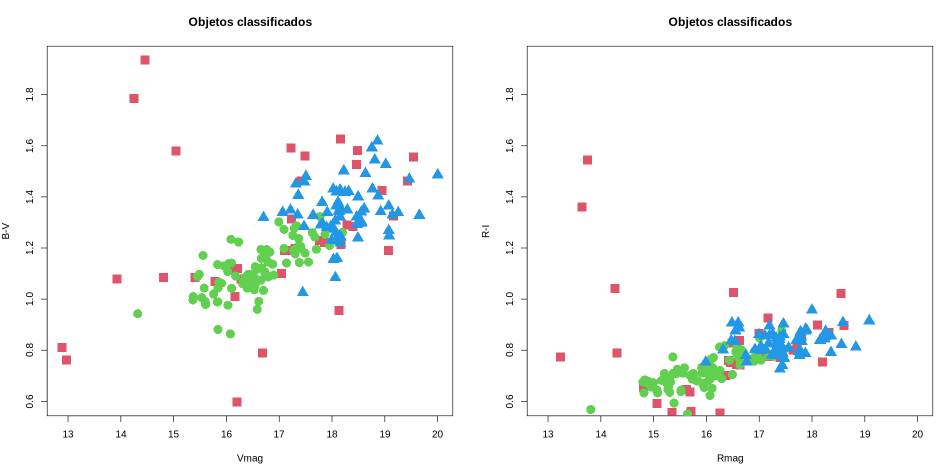
\includegraphics[width=0.8\linewidth]{Figuras/mistura.png}
    \caption{Estrelas do aglomerado aberto King 5 em dois diagramas cor x magnitude. As cores mostram o grupo classificado pela separação de misturas usando o mclust.}
    \label{misturas}
\end{figure}

\textcolor{red}{c) Podemos ver que de fato há 2 populações na imagem \ref{misturas}, onde os objetos do grupo em azul são estrelas mais avermelhadas e com menor brilho aparente, enquanto que o grupo verde são estrelas mais azuladas e maior brilho aparente. Como é um aglomerado e as estrelas devem estar aproximadamente a mesma distância, podemos dizer que esse gráfico se aproxima bastante de um diagrama HR do aglomerado. O terceiro grupo parece ser construídos de outliers, possivelmente objetos fora do aglomerado ou estrelas fora da sequência principal.}

\begin{lstlisting}
    options(repr.plot.width=16,repr.plot.height=8)
    par(mfrow=c(1,2))
    plot(c(), xlim=range(new_df$Vmag), ylim=range(new_df$Bmag - new_df$Vmag),
         xlab="Vmag", ylab="B-V", main="Objetos classificados")
    for (i in c(1:3)){
      sub_df = new_df[model$classification==i,]
      points(sub_df$Vmag,sub_df$Bmag-sub_df$Vmag, col=1+i, pch=14+i,cex=2)
    }
    
    plot(c(), xlim=range(new_df$Vmag), ylim=range(new_df$Bmag - new_df$Vmag),
         xlab="Rmag", ylab="R-I", main="Objetos classificados")
    for (i in c(1:3)){
      sub_df = new_df[model$classification==i,]
      points(sub_df$Rmag,sub_df$Rmag-sub_df$Imag, col=1+i, pch=14+i,cex=2)
    }
\end{lstlisting}



\newpage
{$\space$\par}
\vspace{0.5cm}
\justifying
\section*{{\bfseries \LARGE Questão 8 -} {\bfseries \large  Usando uma abordagem paramétrica e outra não paramétrica, calcule o coeficiente de correlação entre o desvio para o vermelho e a magnitude V, para as galáxias Seyfert 1 (SY1)? Qual a abordagem mais correta a ser considerada? Existe alguma base física para a relação encontrada?}}

\vspace{0.8cm}

\textcolor{red}{A abordagem não-paramétrica geralmente é a mais adequada, pois não depende de conhecimentos prévios dos dados. Porém, como veremos na questão 10, não pode-se rejeitar a hipótese de que o redshift e a magnitude seguem uma distribuição Gaussiana e como o teste de Pearson assume Gaussianidade nas variáveis, então podemos usá-lo. Todavia, há poucos objetos na amostra e isso faz com que os testes falhem, incluindo o de Gaussianidade. Logo, eu considero mais correto utilizar o teste não-paramétrico.}
\vspace{0.4cm}

\begin{lstlisting}
    cor.test(sy1$z, sy1$Vmag, method='pearson')
    cor.test(sy1$z, sy1$Vmag, method='spearman')
\end{lstlisting}

\begin{lstlisting}
        Pearson product-moment correlation
    
    data:  sy1$z and sy1$Vmag
    t = 0.92786, df = 5, p-value = 0.3961
    alternative hypothesis: true correlation is not equal to 0
    95 percent confidence interval:
     -0.5198244  0.8818138
    sample estimates:
          cor 
    0.3832664 
\end{lstlisting}

\begin{lstlisting}
        Spearman rank correlation rho
    
    data:  sy1$z and sy1$Vmag
    S = 36.828, p-value = 0.4523
    alternative hypothesis: true rho is not equal to 0
    sample estimates:
          rho 
    0.3423562 
\end{lstlisting}

\vspace{0.4cm}

\textcolor{red}{Desses valores, não podemos rejeitar a hipótese nula de que não existe correlação ($\rho=0$). Existe sim uma relação física entre a magnitude e o redshift, pois com diferentes redshifts, teremos diferentes partes do espectro na banda V. Todavia, essa relação não é linear, já que o fluxo em diferentes partes do espectro de uma galáxia pode aumentar ou diminuir. Assim, é de se esperar que não tenha uma correlação entre as duas quantidades físicas. Por fim, devemos nos lembrar que há poucos dados e isso limita nosso poder de afirmações.}
\newpage
{$\space$\par}
\vspace{0.5cm}
\justifying
\section*{{\bfseries \LARGE Questão 9 -} {\bfseries \large Use 1000 sorteios de bootstrap para definir o intervalo de confiança de 97.5\% para o valor da mediana da distribuição de desvio para o vermelho (z) da amostra de quasares (QSO) e da amostra de Blazares (BLZ).
}}

\vspace{0.8cm}

\textcolor{red}{A técnica de bootstrap é baseada em amostragem com repetição. Dado um número de sorteios, cada sorteio seleciona N objetos dos dados com repetição e então estima a quantidade desejada para cada sorteio. No fim, obtém-se o uma distribuição da quantidade, onde tira-se o intervalo de confiança.}

\vspace{0.4cm}

\begin{lstlisting}
    theta = function(x,i){
      median(x[i])
    }
    qso_boot = boot(qso_z, statistic=theta, R=1000)
    boot.ci(qso_boot, conf=0.975)
\end{lstlisting}

\begin{lstlisting}
    BOOTSTRAP CONFIDENCE INTERVAL CALCULATIONS
    Based on 1000 bootstrap replicates
    
    CALL : 
    boot.ci(boot.out = qso_boot, conf = 0.975)
    
    Intervals : 
    Level      Normal              Basic         
    97.5%   ( 0.1124,  0.4421 )   ( 0.0763,  0.4080 )  
    
    Level     Percentile            BCa          
    97.5%   ( 0.1770,  0.5087 )   ( 0.1710,  0.4860 ) 
\end{lstlisting}


\begin{lstlisting} 
    blz_boot = boot(blz_z, statistic=theta, R=1000)
    boot.ci(blz_boot, conf=0.975)
\end{lstlisting}

\begin{lstlisting}
    BOOTSTRAP CONFIDENCE INTERVAL CALCULATIONS
    Based on 1000 bootstrap replicates
    
    CALL : 
    boot.ci(boot.out = blz_boot, conf = 0.975)
    
    Intervals : 
    Level      Normal              Basic         
    97.5%   ( 0.0370,  0.7308 )   ( 0.0640,  0.6638 )  
    
    Level     Percentile            BCa          
    97.5%   ( 0.0562,  0.6560 )   ( 0.0461,  0.5950 ) 
\end{lstlisting}

\vspace{0.4cm}

\textcolor{red}{Levando o resultado do "Basic", temos que o intervalo de confiança da mediana quasares é menor do que para os blazares. Possivelmente isso é devido ao menor número de dados na amostra de blazares. }
\newpage
{$\space$\par}
\vspace{0.5cm}
\justifying
\section*{{\bfseries \LARGE Questão 10 -} {\bfseries \large  As distribuições de z e Vmag de cada classe (Type) podem ser consideradas gaussianas? Justifique sua resposta com mais de um teste/análise.}}

\vspace{0.8cm}


\begin{lstlisting}
    for (tip in c('QSO', 'SY1', 'BLZ')) {
      subset = data[data$Type == tip, ]
      z = na.omit(subset$z)
      v = na.omit(subset$Vmag)
      cat('Starting', tip, 'type\n\n')
    
    # Redshift
      if (length(z) > 7) {
      ad_z = ad.test(z)
      cvm_z = cvm.test(z)
      cat('p-value from AD test for redshift in',tip,':',ad_z$p.value,'\n')
      cat('p-value from CVM test for redshift in',tip,':',cvm_z$p.value,'\n')
      }
    
      dip = dip.test(z)
      shapiro = shapiro.test(z)
      lillie = lillie.test(z)
      cat('p-value from dip test for redshift in',tip,':',dip$p.value,'\n')
      cat('p-value from Shapiro test for redshift in',tip,':',shapiro$p.value,'\n')
      cat('p-value from Lillie test for redshift in',tip,':',lillie$p.value,'\n','\n')
    
    # V mag
    
      if (length(v) > 7) {
        ad_v = ad.test(v)
        cvm_v = cvm.test(v)
        cat('p-value from AD test for Vmag in', tip, ':', ad_v$p.value, '\n')
        cat('p-value from CVM test for Vmag in', tip, ':', cvm_v$p.value, '\n')
      }
    
      dip = dip.test(v)
      shapiro = shapiro.test(v)
      lillie = lillie.test(v)
      cat('p-value from dip test for Vmag in', tip, ':', dip$p.value, '\n')
      cat('p-value from Shapiro test for Vmag in', tip, ':', shapiro$p.value, '\n')
      cat('p-value from Lillie test for Vmag in', tip, ':', lillie$p.value, '\n', '\n')
      cat('###########################################################\n\n')
    }
\end{lstlisting}

\newpage


\begin{lstlisting}
    Starting QSO type
    
    p-value from AD test for redshift in QSO : 7.681129e-09 
    p-value from CVM test for redshift in QSO : 1.121454e-07 
    p-value from dip test for redshift in QSO : 0.9870413 
    p-value from Shapiro test for redshift in QSO : 1.547669e-06 
    p-value from Lillie test for redshift in QSO : 1.573389e-05 
     
    p-value from AD test for Vmag in QSO : 0.03655097 
    p-value from CVM test for Vmag in QSO : 0.05203636 
    p-value from dip test for Vmag in QSO : 0.4685278 
    p-value from Shapiro test for Vmag in QSO : 0.03447447 
    p-value from Lillie test for Vmag in QSO : 0.06412205 
     
    ###########################################################
    
    Starting SY1 type
    

    p-value from dip test for redshift in SY1 : 0.1182018 
    p-value from Shapiro test for redshift in SY1 : 0.4400546 
    p-value from Lillie test for redshift in SY1 : 0.6378789 

    p-value from dip test for Vmag in SY1 : 0.9351645 
    p-value from Shapiro test for Vmag in SY1 : 0.2234065 
    p-value from Lillie test for Vmag in SY1 : 0.2478134 
     
    ###########################################################
    
    Starting BLZ type
    
    p-value from AD test for redshift in BLZ : 0.006366748 
    p-value from CVM test for redshift in BLZ : 0.01736082 
    p-value from dip test for redshift in BLZ : 0.7571165 
    p-value from Shapiro test for redshift in BLZ : 0.003163003 
    p-value from Lillie test for redshift in BLZ : 0.08508485 
     
    p-value from AD test for Vmag in BLZ : 0.06981848 
    p-value from CVM test for Vmag in BLZ : 0.06846265 
    p-value from dip test for Vmag in BLZ : 0.9826913 
    p-value from Shapiro test for Vmag in BLZ : 0.1373625 
    p-value from Lillie test for Vmag in BLZ : 0.119869 
     
    ###########################################################
\end{lstlisting}

\vspace{0.4cm}

\textcolor{red}{Da análise de quasares, pode-se dizer que temos evidência para confirmar que as distribuições de redshift e de magnitude V \textbf{não} seguem uma normal. Apesar do p valor alto em alguns testes, como o dip, estou considerando as diversas características de uma distribuição normal, por isso faço tal afirmação.}

\textcolor{red}{Da análise de Seyfert 1, pode-se dizer que não há evidência para confirmar a refutar a hipótese nula de que as distribuições redshift e da magnitude V seguem uma normal.}

\textcolor{red}{Da análise de blazares, pode-se dizer que temos evidência para confirmar que as distribuições de redshift não segue uma normal. Para a magnitude V, não temos evidência para refutar a hipótese nula.}
\newpage



\end{document}